\documentclass[conference,letterpaper]{IEEEtran}
\usepackage[T1]{fontenc}
\usepackage{amsmath,amssymb,booktabs,array,graphicx,cite}
\usepackage{tikz}
\usetikzlibrary{arrows.meta,positioning,fit}
\usepackage[hidelinks]{hyperref}
\newcommand{\StageVsShuffleOne}{1.462}
\newcommand{\StageVsShuffleEight}{1.552}
\newcommand{\RoundVsShuffleOne}{1.520}
\newcommand{\RoundVsShuffleEight}{1.583}
\newcommand{\RoundVsPqrvOne}{4.742}
\newcommand{\RoundVsPqrvEight}{3.074}
\newcommand{\RoundVsPointerOne}{1.130}
\newcommand{\PointerVsRoundEight}{1.374}
\newcommand{\StageLutPct}{1.129}
\newcommand{\RoundLutPct}{0.898}
\newcommand{\StageFfPct}{1.300}
\newcommand{\RoundFfPct}{4.755}
\newcommand{\SharedLutPct}{4.430}
\newcommand{\SharedFfPct}{4.138}
\newcommand{\SharedStageLutPct}{2.231}
\newcommand{\SharedStageFfPct}{1.622}
\newcommand{\AllStageOne}{9.408}
\newcommand{\AllStageEight}{12.909}
\newcommand{\FusionOne}{3.168}
\newcommand{\FusionEight}{3.291}
\newcommand{\StagePermPct}{4.964}
\newcommand{\StageSpongePct}{11.661}
\newcommand{\RoundPermPct}{1.266}
\newcommand{\RoundSpongePct}{12.902}
\newcommand{\DsaPointwiseXrtSaved}{12.538}
\newcommand{\DsaPointwiseEightSaved}{11.687}
\newcommand{\DsaPointwiseEightParity}{0.593}
\newcommand{\KemFinalProbePct}{6.398}
\newcommand{\DsaFinalProbePct}{0.666}
\newcommand{\BankEightNttPenalty}{0.181}
\newcommand{\BankFourNttPenalty}{0.715}
\newcommand{\BankTwoNttPenalty}{2.963}
\newcommand{\BankOneNttPenalty}{25.043}
\newcommand{\BankTwoNttLutSaved}{70.917}
\newcommand{\BankTwoNttFfSaved}{45.954}
\newcommand{\BankTwoNttDspSaved}{87.500}
\newcommand{\BankTwoCoreLutSaved}{4.206}
\newcommand{\BankTwoCoreFfSaved}{4.270}
\newcommand{\BankTwoCoreDspSaved}{39.773}
\newcommand{\BankTwoEndToEndMax}{0.143}
\newcommand{\BankParityMax}{0.959}
\newcommand{\KemNttSaved}{4.913}
\newcommand{\DsaNttSaved}{5.939}
\newcommand{\SharedParityMax}{0.879}
\newcommand{\FusionKemOne}{1.028}
\newcommand{\FusionKemEight}{1.033}

\newcommand{\Mont}{\operatorname{Mont}}
\newcommand{\Barrett}{\operatorname{Barrett}}
\newcommand{\Rot}{\operatorname{ROL}_{64}}
\newcommand{\code}[1]{\texttt{#1}}
\makeatletter
\newcommand{\tablerows}[1]{\@@input #1 }
\makeatother
\hypersetup{pdftitle={Warp-Resident NTT and Keccak Collectives for ML-KEM on a RISC-V GPU},
pdfauthor={Anonymous authors},pdfsubject={Independent six-page IEEE working manuscript}}

\title{Warp-Resident NTT and Keccak Collectives\\for ML-KEM on a RISC-V GPU}
\author{\IEEEauthorblockN{Anonymous Authors}}

\begin{document}
\maketitle
\begin{abstract}
ML-KEM combines polynomial butterflies with Keccak reductions and permutations,
creating different communication demands within one cryptographic request.
We implement collective instructions that operate on ordinary lane registers
of a RISC-V SIMT GPU and retain single-destination writeback. NTT uses XOR-paired
butterflies and a shared 16-multiplier bank; Keccak uses a 25-lane state with
stage or whole-round operations. On a common RV32IM core, cycle-accurate XRT
simulation shows that stage and round instructions accelerate complete
ML-KEM-768 by \StageVsShuffleOne{}--\StageVsShuffleEight{}$\times$ and
\RoundVsShuffleOne{}--\RoundVsShuffleEight{}$\times$, respectively, over the
same software shuffle mapping at one and eight requests. Round fusion improves
the expanded stage permutation by 3.29$\times$, but a separate matched SimX
control shows only about 3\% improvement for complete requests. Independently routed stage
and round extensions add \StageLutPct{}\% and \RoundLutPct{}\% core LUTs over
an NTT-equipped baseline at 250 MHz. These results show why collective
granularity must be selected using complete requests and concurrency, rather
than primitive instruction count alone.
\end{abstract}
\begin{IEEEkeywords}
ML-KEM, Keccak, NTT, SIMT, RISC-V, instruction-set extension
\end{IEEEkeywords}

\section{Introduction}
ML-KEM standardizes a module-lattice key-encapsulation mechanism whose
implementation combines number-theoretic transforms (NTTs), polynomial
arithmetic, sampling, and SHA-3/SHAKE~\cite{fips203,fips202}. These operations
expose substantial parallelism, but their communication differs. An NTT
butterfly exchanges a pair of coefficients and applies a modular product.
A Keccak round reduces columns of a $5\times5$ state, permutes words, and
combines neighboring words. Mapping both to independent scalar lanes leaves
structured communication to software; sending complete operations to a
memory-coupled engine introduces a different state-transfer boundary.

An extensible SIMT processor permits a third option: keep the state in the
warp's ordinary registers and expose the required communication through
collective instructions. However, register residence alone does not determine
the useful instruction size. A larger operation reduces issue demand but
requires more pipeline state, while its application benefit depends on the
remaining sponge, arithmetic, and control work. Concurrent requests can also
change which execution interface is fastest.

We investigate this design space on Vortex, an open RISC-V
GPU~\cite{vortex}. Our design distinguishes \emph{where state resides},
\emph{which lanes cooperate}, and \emph{how much computation one instruction
performs}. For NTT, a strided register layout separates three local levels
from four cross-lane levels. A pair collective computes one modular product
and returns the two butterfly outputs through the lanes' normal destinations.
For Keccak, a 25-lane layout supports either three stage operations or a
complete round. RV32 explicitly selects low and high output halves; RV64
returns whole words. Neither form requires persistent hidden accelerator
state between instructions.

The goal is a realizable SIMT interface, not a claim that these state layouts
or whole-round arithmetic are new. CPU register-coupled cryptographic
extensions already exist~\cite{risqv,nannipieri}; ML-Cube uses 25-thread
Keccak with shuffles~\cite{mlcube}; and a published patent application
describes warp-collective Keccak rounds~\cite{collectivepatent}. We instead
make the operand, participation, and writeback contracts explicit, implement
them in processor RTL, and evaluate their resource and application tradeoffs.

This paper makes three contributions:
\begin{enumerate}
\item A register interface that fits multi-input/multi-output cryptographic
operations into ordinary SIMT operands: pair-low twiddle selection and
distributed butterfly outputs for NTT, and explicit output-half selection
for 25-lane Keccak, all with one destination per lane.
\item Data paths matched to these structures: a statically routed NTT unit
sharing 16 multipliers across 32 lanes, and stage/round Keccak pipelines
using the existing operand and result interfaces.
\item A controlled evaluation separating software mapping, instruction
acceleration, fusion, and batching. Complete ML-KEM reveals diminishing
fusion returns and a latency/throughput crossover with a pointer engine;
post-route implementation quantifies the cost of each register interface.
\end{enumerate}

\begin{figure*}[t]
\centering\resizebox{\textwidth}{!}{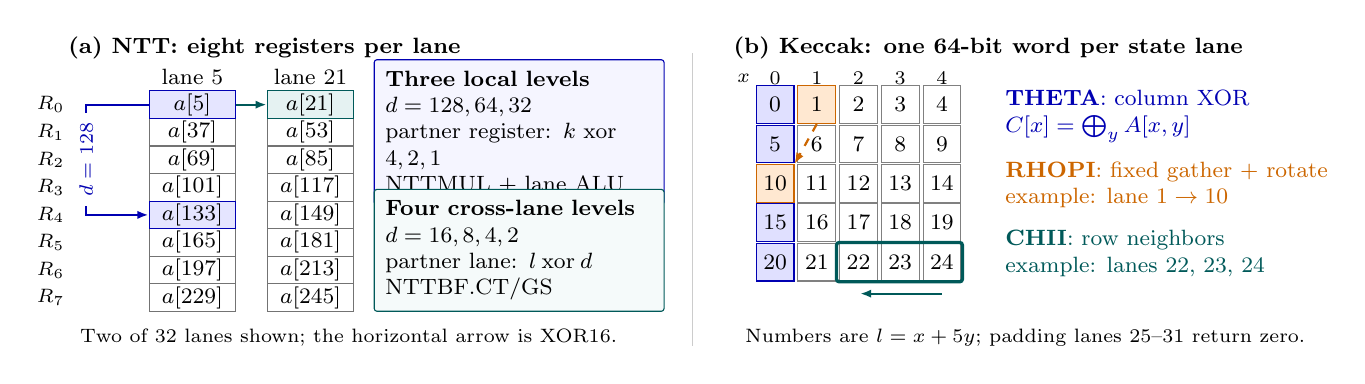
\begin{tikzpicture}[
  font=\footnotesize,
  coeff/.style={draw=black!55,minimum width=11mm,minimum height=3mm,inner sep=1pt},
  block/.style={draw,rounded corners=1pt,align=left,text width=34mm,inner sep=4pt},
  arr/.style={-{Latex[length=1.4mm]},thick}]
\node[anchor=west,font=\footnotesize\bfseries] at (-.7,.72) {(a) NTT: eight registers per lane};
\node at (1.0,.35) {lane 5};
\node at (2.5,.35) {lane 21};
\foreach \k in {0,...,7} {
  \pgfmathtruncatemacro{\a}{5+32*\k}
  \pgfmathtruncatemacro{\b}{21+32*\k}
  \node[font=\scriptsize] at (-.8,-.35*\k) {$R_{\k}$};
  \node[coeff] (left\k) at (1,-.35*\k) {$a[\a]$};
  \node[coeff] (right\k) at (2.5,-.35*\k) {$a[\b]$};
}
\node[coeff,fill=blue!10,draw=blue!70!black] at (1,0) {$a[5]$};
\node[coeff,fill=blue!10,draw=blue!70!black] at (1,-1.4) {$a[133]$};
\node[coeff,fill=teal!10,draw=teal!70!black] at (2.5,0) {$a[21]$};
\draw[arr,blue!70!black] (left0.west) -- (-.35,0) |- (left4.west);
\node[rotate=90,font=\scriptsize,fill=white,text=blue!70!black] at (-.35,-.7) {$d=128$};
\draw[arr,teal!70!black] (left0.east) -- (right0.west);
\node[block,draw=blue!70!black,fill=blue!4] at (5.15,-.35)
  {\textbf{Three local levels}\\$d=128,64,32$\\partner register: $k\mathbin{\mathrm{xor}}4,2,1$\\NTTMUL + lane ALU};
\node[block,draw=teal!70!black,fill=teal!4] at (5.15,-1.85)
  {\textbf{Four cross-lane levels}\\$d=16,8,4,2$\\partner lane: $l\mathbin{\mathrm{xor}}d$\\NTTBF.CT/GS};
\node[anchor=west,font=\scriptsize] at (-.55,-2.96)
  {Two of 32 lanes shown; the horizontal arrow is XOR16.};

\draw[black!20] (7.35,.65) -- (7.35,-3.06);
\node[anchor=west,font=\footnotesize\bfseries] at (7.75,.72) {(b) Keccak: one 64-bit word per state lane};
\foreach \x in {0,...,4} {
  \node[font=\scriptsize] at (8.4+.53*\x,.33) {$\x$};
  \foreach \y in {0,...,4} {
    \pgfmathtruncatemacro{\l}{\x+5*\y}
    \node[draw=black!50,minimum size=4.8mm,inner sep=0pt] (K\l)
      at (8.4+.53*\x,-.5*\y) {\l};
  }
}
\node[font=\scriptsize] at (8.0,.33) {$x$};
\foreach \y in {0,...,4} {
  \pgfmathtruncatemacro{\l}{5*\y}
  \node[fill=blue!12,draw=blue!70!black,minimum size=4.8mm,inner sep=0pt]
    at (8.4,-.5*\y) {\l};
}
\foreach \l in {1,10} {
  \node[fill=orange!18,draw=orange!80!black,minimum size=4.8mm,inner sep=0pt] at (K\l) {\l};
}
\draw[arr,orange!80!black,dashed] (K1.south) -- (K10.north east);
\draw[teal!70!black,very thick,rounded corners=1pt] (9.18,-2.25) rectangle (10.78,-1.75);
\draw[arr,teal!70!black] (10.52,-2.4) -- (9.48,-2.4);
\node[anchor=west,align=left,text=blue!70!black] at (11.2,-.15)
  {\textbf{THETA}: column XOR\\$C[x]=\bigoplus_y A[x,y]$};
\node[anchor=west,align=left,text=orange!80!black] at (11.2,-1.02)
  {\textbf{RHOPI}: fixed gather + rotate\\example: lane $1\rightarrow10$};
\node[anchor=west,align=left,text=teal!70!black] at (11.2,-1.89)
  {\textbf{CHII}: row neighbors\\example: lanes 22, 23, 24};
\node[anchor=west,font=\scriptsize] at (7.9,-2.96)
  {Numbers are $l=x+5y$; padding lanes 25--31 return zero.};
\end{tikzpicture}
}
\caption{The communication structure determines the collective's scope.
(a) NTT changes register index at its first three levels and lane index at
its last four. (b) Keccak combines column reduction, fixed gather/rotation,
and row-neighbor logic on a different lane layout. RV32 stores each state
word as low/high GPR values.}
\label{fig:layout}
\end{figure*}

\section{Communication and State Placement}
\subsection{Two primitives, two participation patterns}
For the ML-KEM modulus $q=3329$, a 256-coefficient forward NTT has seven
levels, with butterfly distances $128,64,32,16,8,4,2$. A 32-thread warp
distributes the polynomial as
\begin{equation}
R_k[l]=a[l+32k],\qquad 0\leq l<32,\quad 0\leq k<8.
\label{eq:layout}
\end{equation}
Figure~\ref{fig:layout} contrasts the two state layouts and their communication.
At the first three levels, partners occupy different registers in the same
lane. At the remaining levels, the partner is lane $l\mathbin{\mathrm{xor}}d$
in the same register vector. There is no distance-one level in ML-KEM.
Contiguous loads/stores for each $k$ surround the transform; the computation
can retain all eight coefficients in lane registers between levels.

Keccak-f[1600] instead has 25 words of 64 bits and 24 rounds. Lane
$l=x+5y$ holds $A[x,y]$, $0\leq x,y<5$. Its column parity, fixed word
permutation, and row-neighbor dependencies involve different lane sets from
the NTT. Lanes 25--31 contain no state, so only 25/32 of the lane positions
represent words. On RV32, each word occupies two GPR values; on RV64, one.
These are state-storage counts, not the peak temporary-register requirement.

\subsection{Why both software and hardware boundaries matter}
Three baselines answer different questions. Scalar C and optimized PQRV
assembly~\cite{pqrv} establish the cost of assigning Keccak to one lane.
A software 25-lane shuffle implementation separates the benefit of the
cooperative mapping from the benefit of new instructions. A pointer engine
accepts a 200-byte state address, executes the complete permutation, and
writes the state back through the memory path. It tests a coarser execution
boundary rather than a different implementation of the same register opcode.

Software cooperation is not uniformly best when implemented with shuffles.
For NTT, a software mapping that groups levels as $3+3+1$ with shared-memory
transposes is stronger than the direct-shuffle version in our archived
pre-extension tests. We retain this denominator when evaluating NTT, rather
than assigning all improvements over a weaker mapping to hardware. Similarly,
one Keccak state per warp is a controlled occupancy point; scalar and
five-lane software can pack more independent states into a warp.

\section{Register Collective Architecture}
Figure~\ref{fig:architecture} relates the layouts to their execution paths.
The arithmetic units are separate. They share the processor's ordinary
operand/result interfaces, not a common modular/Boolean data path or a
demonstrated physical implementation of the general shuffle network.

\begin{figure*}[t]
\centering
\resizebox{.90\textwidth}{!}{%
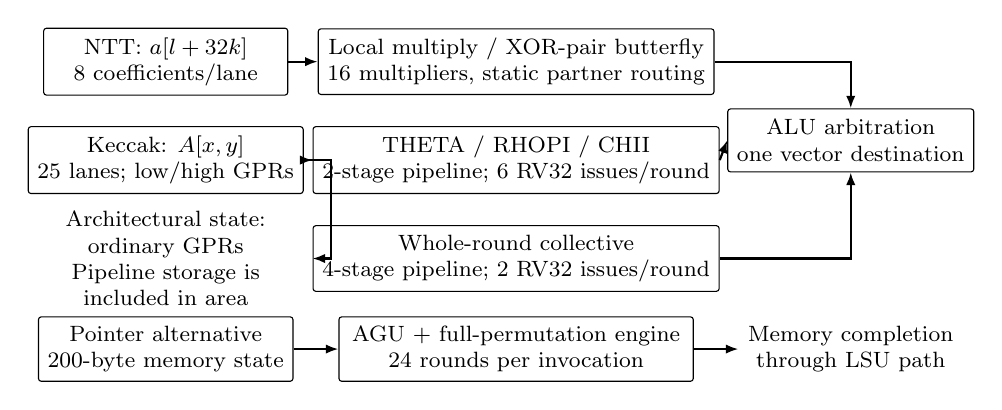
\begin{tikzpicture}[
box/.style={draw,rounded corners=1pt,align=center,font=\footnotesize,minimum height=8mm},
arr/.style={-{Latex[length=1.6mm]},thick},
lab/.style={font=\footnotesize,align=center}]
\node[box,minimum width=31mm] (nstate) at (0,1) {NTT: $a[l+32k]$\\8 coefficients/lane};
\node[box,minimum width=31mm] (kstate) at (0,-.25) {Keccak: $A[x,y]$\\25 lanes; low/high GPRs};
\node[box,minimum width=45mm] (ntt) at (4.45,1) {Local multiply / XOR-pair butterfly\\16 multipliers, static partner routing};
\node[box,minimum width=45mm] (stage) at (4.45,-.25) {THETA / RHOPI / CHII\\2-stage pipeline; 6 RV32 issues/round};
\node[box,minimum width=45mm] (round) at (4.45,-1.5) {Whole-round collective\\4-stage pipeline; 2 RV32 issues/round};
\node[box,minimum width=26mm] (wb) at (8.7,0) {ALU arbitration\\one vector destination};
\draw[arr] (nstate) -- (ntt);
\draw[arr] (kstate) -- (stage);
\draw[arr] (kstate.east) -- ++(.35,0) |- (round.west);
\draw[arr] (ntt.east) -- ++(.4,0) -| (wb.north);
\draw[arr] (stage.east) -- (wb.west);
\draw[arr] (round.east) -- ++(.4,0) -| (wb.south);
\node[lab,text width=32mm] at (0,-1.5) {Architectural state:\\ordinary GPRs\\Pipeline storage is included in area};
\node[box,minimum width=31mm] (mem) at (0,-2.65) {Pointer alternative\\200-byte memory state};
\node[box,minimum width=45mm] (pe) at (4.45,-2.65) {AGU + full-permutation engine\\24 rounds per invocation};
\node[lab] (done) at (8.7,-2.65) {Memory completion\\through LSU path};
\draw[arr] (mem) -- (pe);
\draw[arr] (pe) -- (done);
\end{tikzpicture}}
\caption{Communication-specific execution boundaries. NTT uses lane-local
and pair operations; Keccak Stage and Round are alternative collective
granularities. The pointer baseline transfers state through memory.
Issue counts are architectural operations, not dependent instruction cycles.}
\label{fig:architecture}
\end{figure*}

\subsection{Paired NTT with one result per lane}
\code{NTTMUL.K} performs signed narrow Montgomery multiplication, with
$R=2^{16}$ and modulus 3329. It supports the three lane-local NTT levels,
inverse scaling, and the products in cooperative polynomial arithmetic.
For a cross-lane operation, let $p$ denote the pair-low lane and
$h=p\mathbin{\mathrm{xor}}2^s$ the pair-high lane. The first source vector
supplies $a$ and $b$ at these positions; the second source at $p$ supplies
the twiddle $\zeta$. The CT collective computes
\begin{equation}
t=\Mont(b\zeta),\qquad (r_p,r_h)=(a+t,a-t).
\end{equation}
Only one modular product is needed for the pair. Both lanes write their
own destination, resolving a butterfly's three-input/two-output structure
without a multi-destination instruction. The GS inverse form implements the
library's sign convention:
\begin{equation}
(r_p,r_h)=\bigl(\Barrett(a+b),\Mont((b-a)\zeta)\bigr).
\end{equation}
Sums and differences wrap to signed 16 bits before reduction, matching
the reference's finite-width behavior. The equations do not imply
unbounded intermediate integers.

The instruction encodes $s\in\{0,1,2,3,4\}$. ML-KEM uses $s=4,3,2,1$,
eight instructions per cross-lane level and 32 per transform direction.
Both members of an enabled pair must participate; a partial mask is legal
when every selected pair is either fully active or fully inactive. The supported data path
has 32 ALU lanes and converged participating threads; narrower packetized ALUs would require
additional operand collection and are outside this implementation.

Figure~\ref{fig:pair} shows the concrete CT operation at distance 16.
Lane 5 owns coefficient $a[5+32k]$ and the twiddle, while lane 21 owns
$a[21+32k]$. The collective routes both operands to one pair computation
and distributes its results. The pair-high twiddle is ignored; this is an
architectural rule, not a compiler assumption that both twiddle operands
happen to agree. Tests supply different per-lane twiddles to expose violations.

\begin{figure}[t]
\centering
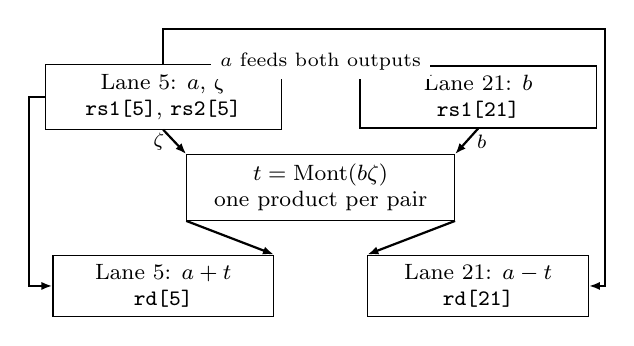
\begin{tikzpicture}[
box/.style={draw,align=center,font=\footnotesize,minimum height=7mm},
arr/.style={-{Latex[length=1.4mm]},thick}]
\node[box,minimum width=30mm] (lo) at (0,0) {Lane 5: $a$, $\zeta$\\\code{rs1[5]}, \code{rs2[5]}};
\node[box,minimum width=30mm] (hi) at (4,0) {Lane 21: $b$\\\code{rs1[21]}};
\node[box,minimum width=34mm] (mul) at (2,-1.15) {$t=\Mont(b\zeta)$\\one product per pair};
\node[box,minimum width=28mm] (outlo) at (0,-2.4) {Lane 5: $a+t$\\\code{rd[5]}};
\node[box,minimum width=28mm] (outhi) at (4,-2.4) {Lane 21: $a-t$\\\code{rd[21]}};
\draw[arr] (lo.south) -- node[left,font=\scriptsize] {$\zeta$} (mul.north west);
\draw[arr] (hi.south) -- node[right,font=\scriptsize] {$b$} (mul.north east);
\draw[arr] (mul.south west) -- (outlo.north east);
\draw[arr] (mul.south east) -- (outhi.north west);
\draw[arr] (lo.west) -- ++(-.2,0) |- (outlo.west);
\draw[arr] (lo.north) -- ++(0,.45) -| ([xshift=2mm]outhi.east) -- (outhi.east);
\node[font=\scriptsize,fill=white] at (2,.45) {$a$ feeds both outputs};
\end{tikzpicture}
\par\smallskip
{\footnotesize
\begin{tabular}{@{}lll@{}}
\toprule
16-multiplier bank & First phase & Second phase\\
\midrule
CT & $b\zeta$ for 16 pairs & ---\\
GS & $(b-a)\zeta$ & $(a+b)20159$\\
NTTMUL & lanes 0--15 & lanes 16--31\\
\bottomrule
\end{tabular}}
\caption{NTT pair computation and bank reuse. At XOR16, lanes 5 and 21
each write their own destination using the pair-low twiddle. Sixteen such
pairs cover W32. CT needs one bank phase; GS and NTTMUL need two.
Phases describe multiplier admission, not complete instruction latency.}
\label{fig:pair}
\end{figure}

The final unit assigns each pair to one of 16 signed $16\times16$
multipliers. Static routing for the five encoded XOR distances avoids
implementing an arbitrary partner permutation. Pair CT uses one product per
bank element. GS reuses the bank first for $(b-a)\zeta$ and then for the
Barrett-quotient product $(a+b)20159$. Lane-local multiplication processes
the lower and upper 16-lane halves in consecutive phases. With registered reduction and result stages,
CT has direct latency/initiation interval 6/1 cycles; GS and a full W32
\code{NTTMUL.K} have 7/2. The result interface preserves the original lane
positions and metadata under backpressure. These unit-level figures do not
include core scheduling, operand hazards, or result arbitration.

\subsection{Stage and round Keccak without hidden state}
The Stage design exposes THETA, RHOPI, and CHII/IOTA. Writing all coordinates
modulo five, its communication is
\begin{align}
C[x]&=\bigoplus_{y=0}^{4}A[x,y],\\
T[x,y]&=A[x,y]\oplus C[x-1]\oplus\Rot(C[x+1],1),\\
B[y,2x+3y]&=\Rot(T[x,y],\rho[x,y]),\\
U[x,y]&=B[x,y]\oplus(\neg B[x+1,y]\land B[x+2,y]).
\end{align}
IOTA XORs the round constant into lane zero. THETA needs a column reduction;
RHOPI needs a fixed gather and rotation; CHII needs two neighboring row
words. Fixed connections implement these dependencies directly.

On RV32, THETA and RHOPI read the old low/high state vectors and return
one selected half. The rotation crosses the half-word boundary, so two
independent 32-bit operations would be incorrect. CHII operates on one half
at a time and takes a uniform round index as its second source. Six
instructions implement one round. Both halves of a stage must read the
same old state, so temporaries prevent the first destination from destroying
an operand of the second instruction. The all-stage permutation loop uses
five GPRs including control and temporaries and has no loads, stores, calls,
or stack frame in its disassembly.

The stage unit uses two pipeline stages and has initiation interval one.
The Round alternative fuses column parity, THETA, RHOPI, and CHII/IOTA into
four registered stages, also with initiation interval one. Each RV32
\code{KROUND.L/H} instruction reads the complete old state and computes its
selected output half; the pair recomputes from identical operands rather
than retaining hidden state for a later high-half write. The literal round
index is encoded in the instruction, producing 48 issues per permutation
instead of Stage's 144. Ordinary hazards and writeback arbitration remain.

Figure~\ref{fig:keccak-issue} shows the RV32 dependencies. Both output-half
instructions read the same old state; the first must not overwrite an
operand needed by the second. Each issue carries its own warp/destination
metadata, so different warps may interleave without an implicit low/high
transaction or private context bank. The RV64 comparison measures whether
removing this half-word interface improves the application.

\begin{figure}[t]
\centering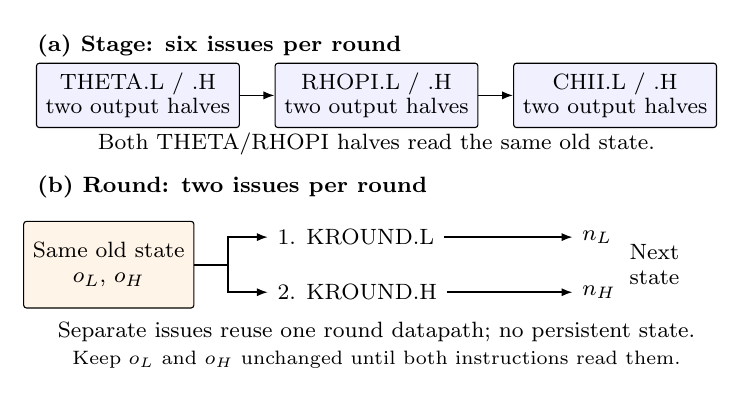
\begin{tikzpicture}[
  x=1cm,y=1cm,
  font=\fontsize{8}{9}\selectfont,
  box/.style={draw,rounded corners=1pt,align=center,minimum height=8mm},
  flow/.style={-{Latex[length=1.4mm]},semithick},
  title/.style={anchor=west,font=\fontsize{8}{9}\selectfont\bfseries},
  op/.style={align=left,anchor=west,font=\fontsize{8}{9}\selectfont}]
\path[use as bounding box] (0,0) rectangle (8.85,4.35);
\node[title] at (0,4.12) {(a) Stage: six issues per round};
\node[box,fill=blue!6,minimum width=25mm] (theta) at (1.40,3.49)
  {THETA.L / .H\\two output halves};
\node[box,fill=blue!6,minimum width=25mm] (rhopi) at (4.43,3.49)
  {RHOPI.L / .H\\two output halves};
\node[box,fill=blue!6,minimum width=25mm] (chii) at (7.46,3.49)
  {CHII.L / .H\\two output halves};
\draw[flow] (theta) -- (rhopi);
\draw[flow] (rhopi) -- (chii);
\node[align=center] at (4.43,2.87)
  {Both THETA/RHOPI halves read the same old state.};

\node[title] at (0,2.33) {(b) Round: two issues per round};
\node[box,fill=orange!9,minimum width=19mm,minimum height=11mm]
  (old) at (1.03,1.34) {Same old state\\$o_L$, $o_H$};
\node[op] (lo) at (3.05,1.69) {1. KROUND.L};
\node[op] (hi) at (3.05,0.99) {2. KROUND.H};
\node[anchor=west] (nextlo) at (6.92,1.69) {$n_L$};
\node[anchor=west] (nexthi) at (6.92,0.99) {$n_H$};
\draw[flow] (old.east) -- ++(.43,0) |- (lo.west);
\draw[flow] (old.east) -- ++(.43,0) |- (hi.west);
\draw[flow] (lo.east) -- (nextlo.west);
\draw[flow] (hi.east) -- (nexthi.west);
\node[anchor=west,align=left] at (7.52,1.34) {Next\\state};
\node[align=center] at (4.43,0.49)
  {Separate issues reuse one round datapath; no persistent state.};
\node[align=center,font=\fontsize{7.5}{8.5}\selectfont] at (4.43,0.13)
  {Keep $o_L$ and $o_H$ unchanged until both instructions read them.};
\end{tikzpicture}

\caption{RV32 issue dependencies for one Keccak round. L/H are separate
issues through one shared unit, each with one vector destination. Stage
uses six issues; Round uses two and recomputes from identical old operands.
The diagram shows dependencies, not simultaneous issue or a cycle schedule.}
\label{fig:keccak-issue}
\end{figure}

All 32 lanes must execute a Keccak collective at the same instruction with
the full mask, including the seven padding lanes, whose outputs are zero.
Guarding execution by \code{lane<25} violates the contract. Loads and stores
can be guarded if lanes reconverge before the collective. Stage's round
operand must be uniform and in $0,\ldots,23$; Round encodes that range.
Simulation assertions and contract tests diagnose invalid participation.

RV64 changes the word interface, not the state distribution: THETA, RHOPI,
and CHII return a complete 64-bit word, and Round needs one issue per round.
The narrow ML-KEM multiplier and butterfly semantics remain unchanged.
Table~\ref{tab:interface} summarizes the resulting contracts.

\begin{table}[t]
\caption{Register collectives. L/H denotes separate RV32 output-half
instructions. All outputs use one destination per participating lane.}
\label{tab:interface}
\centering\footnotesize
\begin{tabular}{@{}lll@{}}
\toprule
Operation & Communication & Output / RV32 issues\\
\midrule
NTTMUL.K & Lane local & One modular product\\
NTTBF.CT/GS & XOR pair & One butterfly / 1\\
THETA.L/H & Five-word column & One stage / 2\\
RHOPI.L/H & Fixed word gather & One stage / 2\\
CHII.L/H & Row neighbors & One stage / 2\\
KROUND.L/H & Complete 25-lane state & One round / 2\\
\bottomrule
\end{tabular}
\end{table}

\subsection{Integrating the complete request}
The ML-KEM integration is based on mlkem-native~\cite{mlkemnative}.
Lane zero executes scalar control, while collective wrappers activate the
warp for NTT, cooperative polynomial arithmetic, and FIPS-202. The wrappers
broadcast arguments, perform the operation, and restore the leader mask.
A request has a shared allocation arena, avoiding 32 redundant allocations
of the same workspace. This integration cost is included in application
timing, rather than eliminated by measuring only an isolated primitive.

One-shot sponge calls retain lane state across absorb, permutation, and
squeeze. Incremental SHAKE saves its context on return and reloads it on
the next call. Thus register residence eliminates transfers \emph{between
primitive stages}, not every state load/store in the complete library. The
pointer alternative loads and stores the 200-byte state on each permutation
invocation through its address-generation and memory path.

\section{Evaluation}
\subsection{Method and comparison boundaries}
The primary platform is one RV32IM core with eight resident warps, 32
threads per warp, and 32-wide ALU/LSU paths. F/D and L2/L3 are disabled;
instruction cache, data cache, and local memory are each 16 KiB. The unified
application experiment enables NTT, Stage, Round, and Pointer in the
\emph{same} XRT runtime and changes only the software Keccak backend.
NTT and cooperative polynomial arithmetic are held fixed.

Each request runs ML-KEM-768 KeyGen, Encaps, and Decaps using the same FIPS
203 known-answer-test inputs. All public/secret keys, ciphertexts, and
encapsulation/decapsulation shared secrets match byte for byte. Each request
performs 140 permutations, 15 NTTs, and nine inverse NTTs. We measure one
request ($M=1$) and eight concurrent requests ($M=8$). For M8, we compare
complete-batch launch cycles, not the sum of overlapping per-request intervals. Reported whole-launch
device cycles include launch/teardown work and exclude host transfers.

XRT simulation exercises both the AFU and processor RTL; it is not a board
measurement. The 12 unified application cases match SimX retired-instruction
counts exactly, with maximum whole-launch cycle difference 2.710\%.
Primitive tests verify coefficients/words, guard regions, pair twiddle
selection, active-mask contracts, and backpressure. Standalone butterfly
validation checks 334,080 outputs across all five distances. Performance
figures use their stated timing scope rather than inferring throughput from
instruction counts.

\begin{figure*}[t]
\centering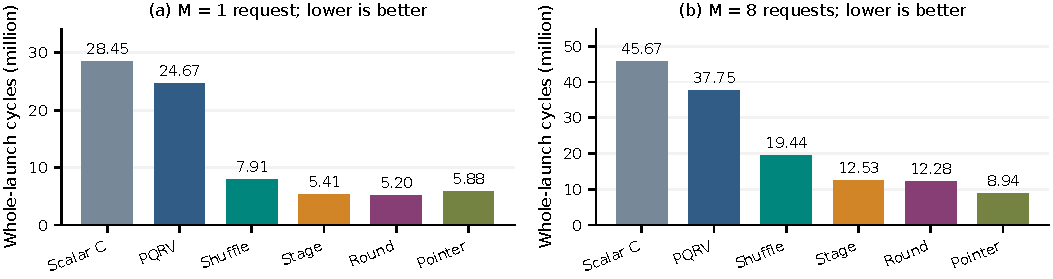
\includegraphics[width=\textwidth]{assets/kem_xrt.pdf}
\caption{Complete ML-KEM-768 on one common RV32IM XRT runtime, with the
final NTT and cooperative arithmetic fixed. All requests pass KAT. Stage
is looped and Round is expanded here; the separate equal-expansion control
isolates fusion. M1 shows latency; M8 shows the time to complete eight requests.}
\label{fig:kem}
\end{figure*}

\subsection{Software mapping and complete-KEM gains}
Figure~\ref{fig:kem} first shows why scalar software is an insufficient
instruction baseline. Moving from PQRV to software SG25 changes M1 cycles
from 24.672 million to 7.909 million and M8 from 37.753 million to 19.440
million, before any Keccak collective instruction is used. Relative to this
same shuffle mapping, Stage improves complete requests by
\StageVsShuffleOne{}$\times$/\StageVsShuffleEight{}$\times$ and Round by
\RoundVsShuffleOne{}$\times$/\RoundVsShuffleEight{}$\times$ at M1/M8.
Against PQRV, Round reaches
\RoundVsPqrvOne{}$\times$/\RoundVsPqrvEight{}$\times$, but those larger
ratios include the software mapping improvement. All these denominators
already use accelerated NTT; they are not combined Keccak-plus-NTT gains
over an unmodified GPU.

The preferred backend changes with concurrency. At M1, Round takes
5.203 million cycles versus Pointer's 5.878 million, a
\RoundVsPointerOne{}$\times$ advantage. At M8, Pointer finishes in 8.939
million cycles versus Round's 12.280 million, a
\PointerVsRoundEight{}$\times$ advantage in the opposite direction.
Register residence therefore does not guarantee the best batch throughput.
The two interfaces create different issue and memory traffic; the observed
crossover establishes a design boundary, but these measurements alone do
not assign it to one specific scheduler or cache mechanism.

\subsection{Fusion improves the primitive more than the application}
Round embeds a literal round index, so its code is expanded. Comparing it
only with looped Stage would also count removed loop overhead. We therefore
expand Stage's 24 rounds and measure the same input/output-isolated interval
with one state per warp and 64 dependent permutations per state.
Figure~\ref{fig:granularity} uses XRT results from that matched control.
With eight active warps, expanded Stage takes 387.354 cycles per completed
permutation and Round takes 117.693, a 3.291$\times$ improvement. For one
active warp, the corresponding ratio is 3.168$\times$.

The application benefit is much smaller. In the matched expansion SimX
control, M1 cycles change from 5,341,994 to 5,198,475 and M8 from
12,336,487 to 11,937,913: only 1.028$\times$ and 1.033$\times$.
These controls use a Stage/Round-enabled core and are kept distinct from
the all-backend XRT experiment. They show that the large primitive gain
survives equal code expansion, but most request time lies elsewhere.

\begin{figure}[t]
\centering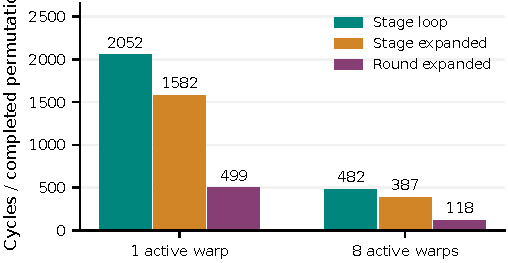
\includegraphics[width=\columnwidth]{assets/granularity.pdf}
\caption{Matched expansion control, XRT: 64 dependent permutations per
state, one state per active warp. Values normalize the isolated span by
completed permutations; they do not represent maximally packed software throughput.}
\label{fig:granularity}
\end{figure}

Separate M1 XRT profiles provide a direct explanation
(Fig.~\ref{fig:profile}). Permutation occupies 4.964\% of the instrumented
Stage request, 1.266\% for Round, and 0.516\% for Pointer. Absorb and squeeze
exclude nested permutation intervals; NTT/INTT contributes approximately
2.1--2.4\%. Remaining work includes sampling, encoding, comparisons, memory,
control, wrappers, and instrumentation. The matched SimX control estimates probe overhead at
6.6--8.3\%, so these intervals explain bottleneck migration but do not
replace the uninstrumented speedup denominator. Further permutation fusion
cannot remove this remaining work.

For scale, an Amdahl-style calculation with Stage's instrumented fraction
$f=0.04964$ and single-warp primitive speedup $s=3.168$ gives
$1/(1-f+f/s)\approx1.035$. This illustrates the small remaining opportunity;
it is not an uninstrumented prediction. At M8, overlapping warps and shared
resources also prevent adding single-request fractions into a batch model.

\begin{figure}[t]
\centering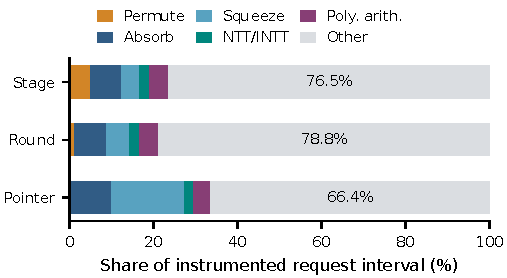
\includegraphics[width=\columnwidth]{assets/phase_profile.pdf}
\caption{Mutually exclusive M1 intervals from independently enabled
RV32IM backends, measured through XRT. ``Other'' is a residual of the
instrumented request, not one cryptographic primitive.}
\label{fig:profile}
\end{figure}

\subsection{NTT communication and multiplier-bank sizing}
We separate the NTT study from the final Keccak sweep because it uses an
earlier matched pointer-enabled core. Holding the full-bank modular
multiplier fixed, replacing software shuffles with pair butterflies reduces
complete-KEM SimX cycles by 2.564\% at M1 and 8.232\% at M8. This comparison
isolates the communication instruction. Against the stronger shared-memory
$3+3+1$ implementation with the same modular-multiply extension, XRT
improvements are smaller: 7,791,578 to 7,711,455 cycles at M1 (1.028\%) and
11,049,301 to 10,522,959 at M8 (4.764\%). These are KEM intervals, not the
whole-launch values of Fig.~\ref{fig:kem}.

\begin{table}[t]
\caption{NTT mapping and bank control, XRT KEM-interval cycles. Historical
matched pointer-enabled core; other operations fixed within this family.}
\label{tab:ntt}
\centering\footnotesize
\begin{tabular}{@{}lrr@{}}
\toprule
NTT implementation & M1 & M8\\
\midrule
Shared transpose + NTTMUL & 7,791,578 & 11,049,301\\
Pair + NTTMUL, 32 multipliers & 7,711,455 & 10,522,959\\
Pair + NTTMUL, 16 multipliers & 7,711,455 & 10,518,691\\
\bottomrule
\end{tabular}
\end{table}

Bank sizing is a separate implementation choice. CT pair butterflies do not
need 32 independent products simultaneously, motivating a 16-multiplier
implementation. A matched full-core post-route comparison reduces LUTs
from 356,447 to 341,680, FFs from 272,430 to 270,865, and DSPs from 192 to
176; both close 250 MHz. The same application ELF changes complete-KEM
cycles by at most 0.041\% across SimX, processor RTL, and XRT at M1/M8
(Table~\ref{tab:ntt} gives the XRT points).
This historical comparison includes floating-point hardware and Pointer;
its absolute area is not combined with the integer-only results below.
It supports the bank choice, not an additional application speedup claim.

\subsection{Full-core area and integer-width sensitivity}
Table~\ref{tab:ppa} reports separate RV32IM implementations of the
NTT-equipped core with each register Keccak extension enabled independently.
All use Vivado 2025.1, the Alveo V80 part, OPT3, a 250 MHz constraint, and
fresh full-core synthesis/place/route. All have zero routing errors, 133
BRAM tiles, and 112 DSPs. They are routed core implementations, not complete
board shells or on-board measurements.

\begin{table}[t]
\caption{Independent RV32IM post-route implementations. F/D disabled,
W8T32, final half-bank NTT; WNS is in ns at 250 MHz.}
\label{tab:ppa}
\centering\footnotesize
\begin{tabular}{@{}lrrrr@{}}
\toprule
Core & LUT & FF & DSP & WNS\\
\midrule
\tablerows{assets/ppa_rows.tex}
\bottomrule
\end{tabular}
\end{table}

Stage adds \StageLutPct{}\% LUTs and \StageFfPct{}\% FFs over NTT only;
Round adds \RoundLutPct{}\% and \RoundFfPct{}\%, respectively. Round's
deeper pipeline increases storage, but its integrated LUT count is slightly
lower than Stage's. Whole-core deltas include integration and placement
effects; the two metrics do not select a universal area winner. The common
runtime performance experiment enables all backends, whereas this table
measures independent area configurations. We therefore do not combine them
into a claimed measured throughput-per-area ranking. A matched integer-only
Pointer implementation is not yet available for this table.

RV64 halves Keccak collective issues but widens more than the primitive.
With F/D disabled on both cores, whole-launch retired instruction counts
for the Stage/Round backends decline only 7.002\%/5.730\%.
M8 XRT cycles change by $-0.403\%$/$+0.180\%$.
The corresponding RV64 cores use 432,843/431,004 LUTs, about 1.94$\times$
the RV32 cores; neither closes the 250 MHz target (WNS
$-0.148$/$-0.013$ ns). These single-run implementation results favor keeping
narrow NTT arithmetic independent of XLEN and evaluating width at complete
core scope. They do not establish a general disadvantage of 64-bit GPUs.

\newpage
\section{Related Work and Scope}
NTT-PIM maps operations according to the location of butterfly partners in
memory buffers~\cite{nttpim}, and BP-NTT co-designs SRAM layout and modular
multiplication~\cite{bpntt}. Our storage and execution domain is the SIMT
GPR bank, with explicit pair participation and normal per-lane writeback.
RISQ-V already demonstrates CPU register-coupled NTT/Keccak
acceleration~\cite{risqv}; Nannipieri et al. integrate scalar NTT arithmetic
extensions into a RISC-V pipeline~\cite{nannipieri}. Register residence,
modular multiplication, and butterfly fusion individually are prior ideas.

ML-Cube's software Keccak layout and the NVIDIA collective-round patent
are particularly close to our 25-lane execution boundary~\cite{mlcube,collectivepatent}.
Our contribution is its concrete RV32/RV64 operand and single-vector
writeback realization together with communication-specific NTT and a
controlled implementation study, not the first such collective concept.
PacQ and SynGPU illustrate related GPU dataflow/hardware co-design for
other workloads~\cite{pacq,syngpu}. CHAM and ZK-Flex motivate evaluating
cryptographic acceleration beyond an individual transform~\cite{cham,zkflex}.
Their different algorithms and platforms preclude direct speedup comparisons.

The evidence here covers ML-KEM-768 at fixed known-answer inputs and two
request counts. It does not establish optimal occupancy, input-distribution
statistics, ML-DSA end-to-end acceleration, activity-based energy, or
side-channel resistance. Constant arithmetic structure and KAT success are
not substitutes for a security evaluation. Additional concurrency points,
input diversity, and board execution would broaden the design conclusions.

\section{Conclusion}
Ordinary warp registers can support both pairwise NTT butterflies and
25-lane Keccak collectives without introducing multi-destination writeback
or persistent hidden accelerator state. Matching the operation to the
communication structure enables a compact NTT bank and practical stage/round
Keccak pipelines. Complete ML-KEM, however, bounds the useful fusion depth:
large primitive gains shrink at application scope, and a pointer engine
can lead at higher concurrency. State placement, instruction granularity,
and request concurrency must therefore be evaluated together.

\section*{Content Generated by AI}
OpenAI Codex assisted with manuscript drafting, literature organization,
and figure-generation code. The draft uses archived experimental results;
author review of the text, citations, and interpretation remains required.

\clearpage
\bibliographystyle{IEEEtran}
\bibliography{references}
\end{document}
